\renewcommand{\chaptername}{March 15th: Lab}
\chapter{Quantum Teleportation}
In quantum teleportation, the properties of quantum entanglement are used to send a qubit between observers without physically moving the involved qubit. The qubits themselves are not really teleported, but the state of one qubit is destroyed on one side and extracted on the other side, so the information that the state encodes is communicated. The process is not instantaneous, because information must be communicated classically between observers as part of the process. The usefulness of quantum teleportation lies in its ability to send quantum information arbitrarily far distances without exposing quantum states to thermal decoherence from the environment or other adverse effects.

This may sound a bit like science fiction, but quantum teleportation can in principle be used to actually teleport macroscopic objects (in the sense that two objects in exactly the same quantum state are identical). However, the number of entangled states necessary to accomplish this is well outside anything physically achievable, since maintaining such a massive number of entangled states without decohering is a difficult problem.

\section{Objectives}

\begin{itemize}
    \item Implement a quantum algorithm
    \item Understand the principles on quantum teleportation and how it can be implemented/applied
\end{itemize}

\section{Methods}

The following qubit state  $|\Psi \rangle = \alpha |0 \rangle + \beta |1 \rangle$ needs to be transferred. This entails passing on information about $\alpha$ and $\beta$. There exists a theorem in quantum mechanics which states that you cannot simply make an exact copy of an unknown quantum state, known as the no-cloning theorem. As a result a copy of  $|\Psi \rangle$ cannot simply be generated (classical states can be copied, not superpositions).

By taking advantage of two classical bits and an entangled qubit pair, the state $|\Psi \rangle$ can be transferred.

This is called teleportation because, at the end, the state $|\Psi \rangle$ will be with the end user and not with the sendee anymore.

\subsection{Teleportation Protocol}
The following steps were followed to create an entanglement protocol and to perform quantum teleportation.

\begin{enumerate}
    \item Use a third party entangled qubit pair
    \item Alice should then perform some operations on her qubit
    \item Then send the results to Bob over a classical communication channel
    \item Bob then performs some operations on his end to receive Alice’s qubit
\end{enumerate}

\section{Results}

The final circuit is shown in Figure \ref{fig:teleportCircuit}
\begin{figure}[h]
    \centering
    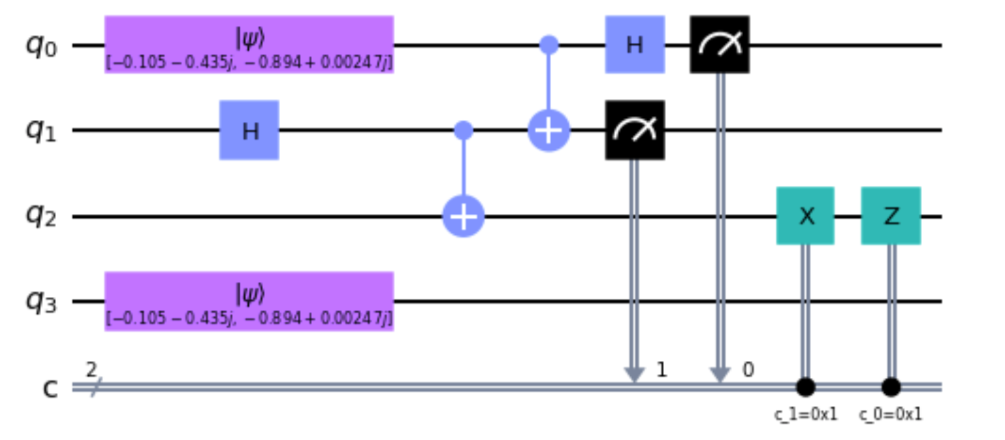
\includegraphics[width=0.6\textwidth]{lab3/teleportCircuit.png}
    \caption{teleportCircuit}
    \label{fig:teleportCircuit}
\end{figure}

\subsubsection{Step 1}
My work

\subsubsection{Step 2}
My work

\subsubsection{Step 3}
My work

\subsubsection{Step 4}
My work

The result from this circuit was observed using Bloch Sphere representation, as seen in Figure \ref{fig:teleportBloch}
\begin{figure}[h]
    \centering
    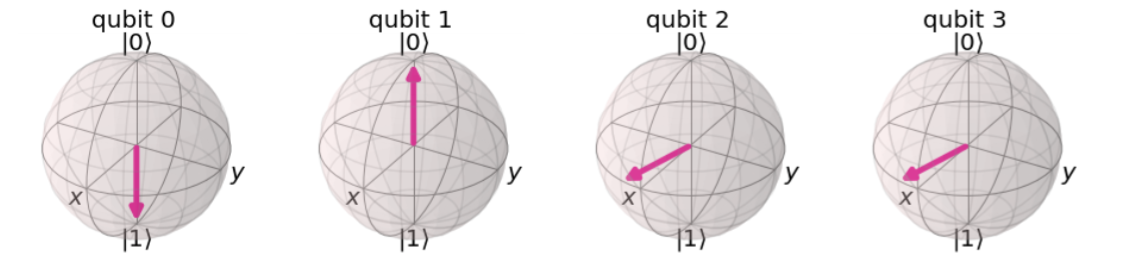
\includegraphics[width=\textwidth]{lab3/teleportBloch.png}
    \caption{teleportBloch}
    \label{fig:teleportBloch}
\end{figure}

To verify the robustness of this design, the circuit was built using IBMs remote quantum computer. The result from which can be seen in Figure \ref{fig:ibmTeleport}
\begin{figure}[h]
    \centering
    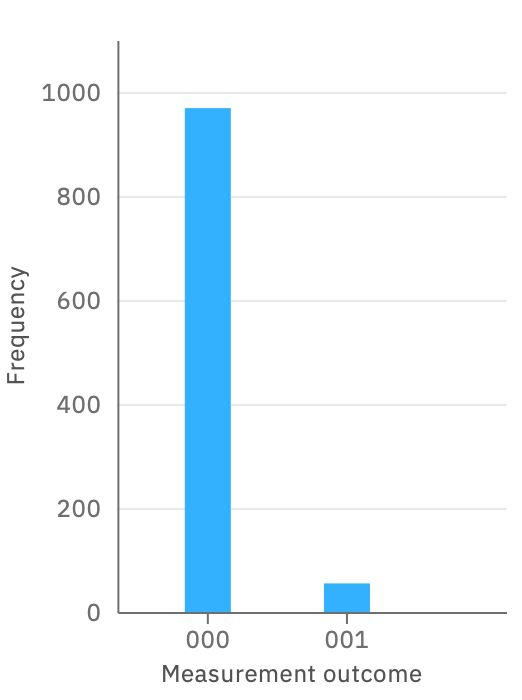
\includegraphics[width=0.38\textwidth]{lab3/ibmTeleport.png}
    \caption{ibmTeleport}
    \label{fig:ibmTeleport}
\end{figure}

\section{Comparison of results with theory}
\section{Discussion}
\textbf{Question 1:}

Follow the steps above, and the knowlege of qiskit you now have from Lab 2 to create an entanglement protocol. You may also benefit from the little revision above which introduce a couple of new features of qiskit

\textbf{Question 2:}

\textbf{2(a)}: Use IBM composer and compare its results to what you obtained above. Are they different? How so?

\textbf{2(b):} Now that you have implemented it, what could quantum telleortation be used for and why is it important?

\section{Conclusions}